
\begin{figure}
\centering

% TODO should mention sizes! Maybe represent decoder output differently.

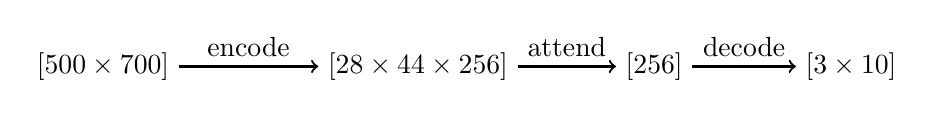
\begin{tikzpicture}
% 900, 1500, 1
% 28, 44, 256
% 1, 1, 256
% 3, 10

    \node (input) at (0,0) {$[500 \times 700]$};
    \node (encoded) at (4, 0) {$[28 \times 44 \times 256]$};
    \node (attended) at (7, 0) {$[256]$};
    \node (decoded) at (9.5, 0) {$[3 \times 10]$};

%   \pic [fill=cyan, draw=blue] at (-1,0) {annotated cuboid={width=1, height=900, depth=1500}};
%   \pic [fill=cyan, draw=blue] at (4,-0.5) {annotated cuboid={width=256, height=28, depth=44}};
%   \pic [fill=cyan, draw=blue] at (7,-0.5) {annotated cuboid={width=256, height=1, depth=1}};
%   \pic [fill=cyan, draw=blue] at (9,1.5) {annotated cuboid={width=1, height=10, depth=3}};

  \draw [->,thick] (input) -- node [above] {encode} (encoded);
  \draw [->,thick] (encoded) -- node [above] {attend} (attended);
  \draw [->,thick] (attended) -- node [above] {decode} (decoded);

\end{tikzpicture}

\caption{Overview of how the data flows in the proposed network. First the encoder produces a matrix of feature vectors, each corresponding to a different but overlapping location in the input image. Secondly, the attention aggregates the feature vectors into a single feature vector. Lastly, the decoder produces three softmax outputs, one for each digit.}
\label{fig:sys_overview}
\end{figure}
